\section{Background Processes}
There are several physics processes that have signatures consistent
with our event selection. The dominant background contribution for
this analysis comes from $Z$ bosons produced in association with jets
(\Zj). The other background contribution comes from
standard model $\ttbar \ra \Wp b \, \Wm \bbar$ events in which the
invariant mass of two leptons in the dilepton decay mode or a lepton
and a jet misidentified as a lepton in the lepton+jets decay mode fall
within the $Z$ mass window. A similar contribution comes from
dibosons which have a real $Z$ in the event ($WZ$, and $ZZ$). Very small 
contributions come from $W$s produced in association with jets (\Wj), and 
from the $WW$ diboson process. In both of those cases, the events do not
have a $Z$ in the final stats, and a lepton from the $W$ decay and a 
misidentified jet from the even are needed to form a $Z$ candidate. 
These backgrounds and the methods for estimating them are described in this
section. The backgrounds from \Wj and $WW$ diboson production is negligible.
Table~\ref{table:bkg_summary} gives a summary of all the backgrounds
and the number of expected events in the signal region from each
background.

\subsection[$Z$ + Jets]{\boldmath $Z$ + Jets\unboldmath}
The dominant source of background for the search for the FCNC decay
\tZq is SM $Z$s produced in association with jets. We use a combination
of the \alp v2.10 MC generator~\cite{Mangano:2002ea}---using \pyth for
parton showers---and data from control regions to estimate the \Zj
background. In general we expect the \alp MC to correctly model the
shapes of kinematic distributions and the relative \xsects between
the different $n$-parton samples. However, \alp underestimates the
overall inclusive $Z$ \xsect because it only generates leading order
diagrams. Therefore we take the overall normalization from inclusive
$Z$'s in the data.

There are two separate sources for $b$-tags in the \Zj sample. We can
get real tags from events with heavy flavor jets and mistagged jets from
events with only light flavor jets.  We estimate how many of the
\Zj events in the signal region will be tagged using both the MC
simulation and data.  We estimate mistags using the
Gen6 mistag parameterization and scale tags by the $b$-tagging scale factor
on a per-jet basis. We measure the $b$-jet tagging fractions in the MC
simulation and check them in data. These numbers are combined to a per-event
tagging probability as described in Section~\ref{section:tageff}.

%We expect 125 events $\pm$ () from \Zj in our signal region and 14 events 
%$\pm$ () with a loose SECVTX tag. 

\subsubsection{Monte Carlo Samples}
We use \alp v2.10 + \pyth MC samples for $Z+0,1,2,3,4$\,partons, and
for two heavy flavor samples, $Z+\bbbar+0,1,2$\,partons, and
$Z+\ccbar+0,1,2$\,partons. \alp v2.10 contains a built-in
mechanism to remove the overlap between jets from parton showers and
from hard scattering matrix elements at the generator level (``MLM
matching''). The samples with the largest parton multiplicities, \ie
$Z+4$\,partons, $Z\bbbar+2$\,partons, and $Z\ccbar+2$\,partons, are
generated using ``inclusive'' matching, hence allowing for processes
with higher parton multiplicities. For all other samples we used
``exclusive'' matching. The samples and their generated \xsects are
listed in Table~\ref{table:Znpsigma}.

The samples are combined according to their generated relative
\xsects.  In the heavy flavor samples, the $b$ and $c$ quarks are
treated as massive objects, while they are massless in the $Z+0,1,
2,3,4$\,parton sample. Unlike for the light flavor samples, there are
no cuts on the minimum separation of two heavy flavor partons. Also, 
heavy flavor partons have a very loose maximum pseudorapidity cut of 
$|\eta|<10$.  Hence we allow for jets that leave the detector undetected 
or jets that contain the daughter particles of more than one $b$ or $c$ quark.  
The heavy quarks contained in the light-flavor sample constitute another overlap
between the samples that is not removed automatically, and we must therefore
remove this overlap by hand. We apply the jet-based
overlap removal scheme developed for the SECVTX top
\xsect analysis~\cite{CDF8767}, as summarized in Table~\ref{table:overlap}.
The guiding idea is that the light flavor samples should not contain
heavy flavor but that collinear \bbbar and \ccbar pairs are simulated
better in \pyth parton showers than in \alp. This leads to a
prescription that keeps \bbbar or \ccbar pairs in the light flavor
sample only if they come from the parton shower (in \pyth: \texttt{STDHEP=2})
and are contained in the same reconstructed jet ($\Delta R<0.4$). In
the heavy flavor samples, all \bbbar and \ccbar pairs from the matrix element
that do not share the same jet are kept.

\begin{table}[t]
  \caption{Heavy flavor overlap removal scheme. Samples marked 'X' are removed, 
    and samples marked 'O' are kept.}
  \small
  \centering
  \vspace{2mm}
  \label{table:overlap}
  \begin{tabular}{c|c|c|c|c|c}
    \toprule
    {\bf Sample} & 
    {\bf No HF} & 
    \multicolumn{2}{|c|}{\bf Matrix Element \boldmath\bbbar/\ccbar\unboldmath} &
    \multicolumn{2}{|c}{\bf Parton Shower \boldmath\bbbar/\ccbar\unboldmath} \\
    & & $\Delta R < 0.4$ & $\Delta R \geq 0.4$ & $\Delta R < 0.4$ & $\Delta R \geq 0.4$ \\
    \midrule
    LF & O & X & X & O & X \\
    \ccbar & --- & X & O & O & O \\
    \bbbar & --- & X & O & O & O \\
    \bottomrule
  \end{tabular}
\end{table}


\subsubsection{Pre-tag Prediction and Mass $\chi^2$}
The distribution of the number of jets in events with a reconstructed
$Z$ obtained from combining the above samples is shown in
Fig.~\ref{fig:zjets}.  Although the sample weights were chosen such
that the samples were normalized to a luminosity of 1.12\invfb, we
cannot use the prediction for number of events with $Z+\geq 4$ jets
directly because \alp as a leading order MC generator underestimates
the inclusive $Z$ \xsect. The \alp v2.10 generated inclusive $Z$
\xsect is around $185\unit{pb}$ whereas the CDF measured \xsect for
$Z\to\ellell$ is $\sigma\times\br(\ppbar\to Z/\gamma^* \to
\ellell)=254.9 \pm 16.2\unit{pb}$~\cite{Acosta:2004uq}.  In order to
get an initial estimate of the number of \Zj background events expected in our signal
region, we normalize our sample to the number of inclusive $Z$
candidates in data. We restrict the normalization to events with three
or fewer jets in order not to unblind the analysis. In the full
dataset of $1.12\invfb$ we find 103,695 events with a $Z$ and three or
fewer jets. \alp predicts the ratio of events with four or more jets
over events with three or fewer jets to approximately 0.001, including
contributions of SM \ttbar and diboson MC.  This yields a first
estimate of approximately 110 events with a $Z$ and four or more jets
in $1.12\invfb$ of data. In the following we will refine this number
using both MC and data-driven techniques.

\begin{figure}[t]
  \begin{center}
    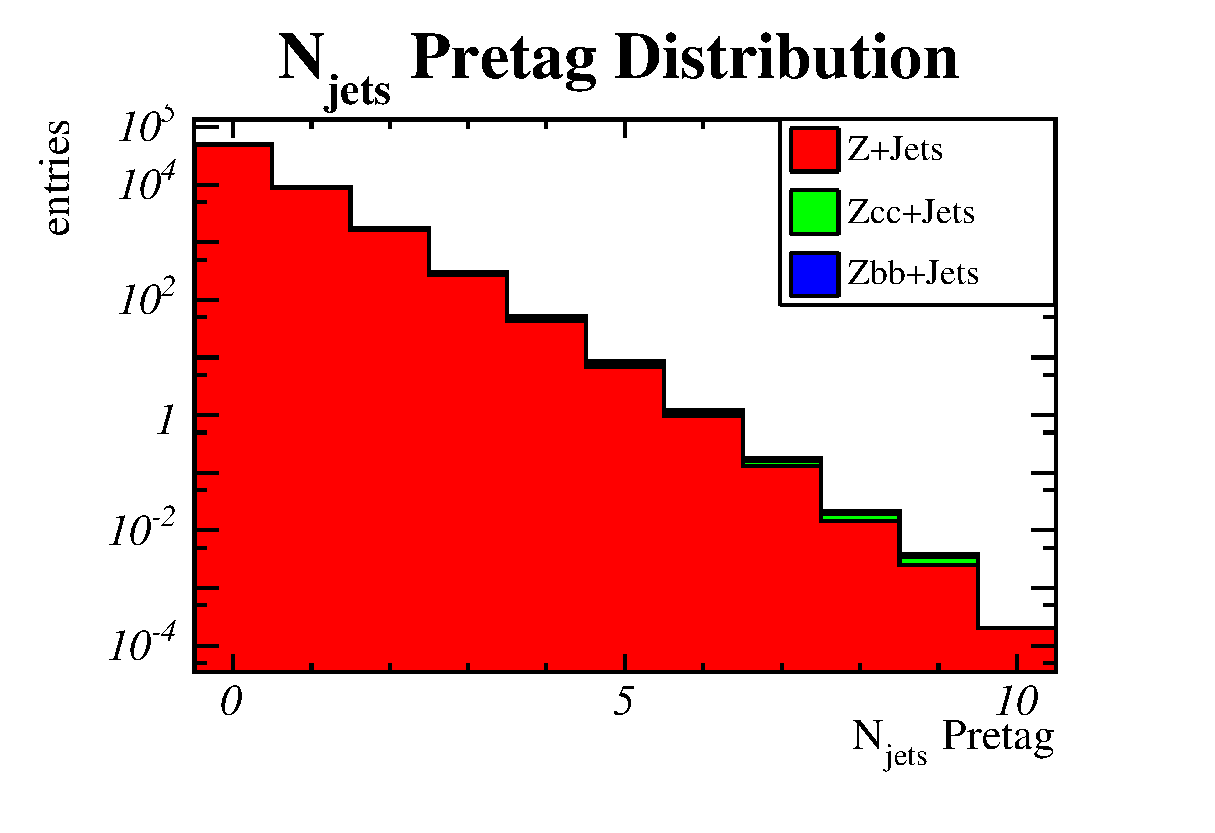
\includegraphics[width=0.6\textwidth]{pics/njet_alpgenonly.eps}
  \end{center}
  \caption{Distribution of the number of jets in events with a
    reconstructed $Z$ from the combination \alp \Zj, SM \ttbar, and
    diboson MC samples.}
  \label{fig:zjets}
\end{figure}

In Fig.~\ref{fig:alpdata}, a comparison of the predictions of the
\alp, SM \ttbar, and dibosons MC samples with data for events with a
$Z$ and three or fewer jets is shown.  The MC simulation
underestimates the number of jets by 15\% already for
$Z+3\:$jets. Therefore we developed a second technique to estimate the
\Zj background that is more data-driven and based on the mass $\chi^2$
described in Section~\ref{section:masschi2}. The separation of signal
from background events as a function of $\chi^2$ is shown in
Fig.~\ref{fig:chi2_separation}. The good separation and the
approximate independence of the background shape of the parton
multiplicity in the \Zj MC leads to the idea of extending the
unblinded area of the analysis to the tail of the $\chi^2$
distribution. For example, a cut of $\sqrt{\chi^2}>3$ would accept
only 3\% of the FCNC signal, but 29\% of the \Zj background. Note that
the $\chi^2$ shape of all background samples is very similar.

As a data-driven method to determine the \Zj background, we fit data
to the high-$chi^2$ tail and extrapolate to the signal region of low
$chi^2$ using the MC shape of the \Zj distribution.  With a cut of
$\sqrt{\chi^2}>3$ we obtain $151 \pm 28$ events, and with a cut of
$\sqrt{\chi^2}>3.2$, the yield is $119 \pm 21$. We take the average of
these two numbers as the background prediction from the mass $\chi^2$,
and the larger of the two uncertainties: $135 \pm 28$ events.


\begin{figure}[t]
  \begin{center}
    \subfigure[]{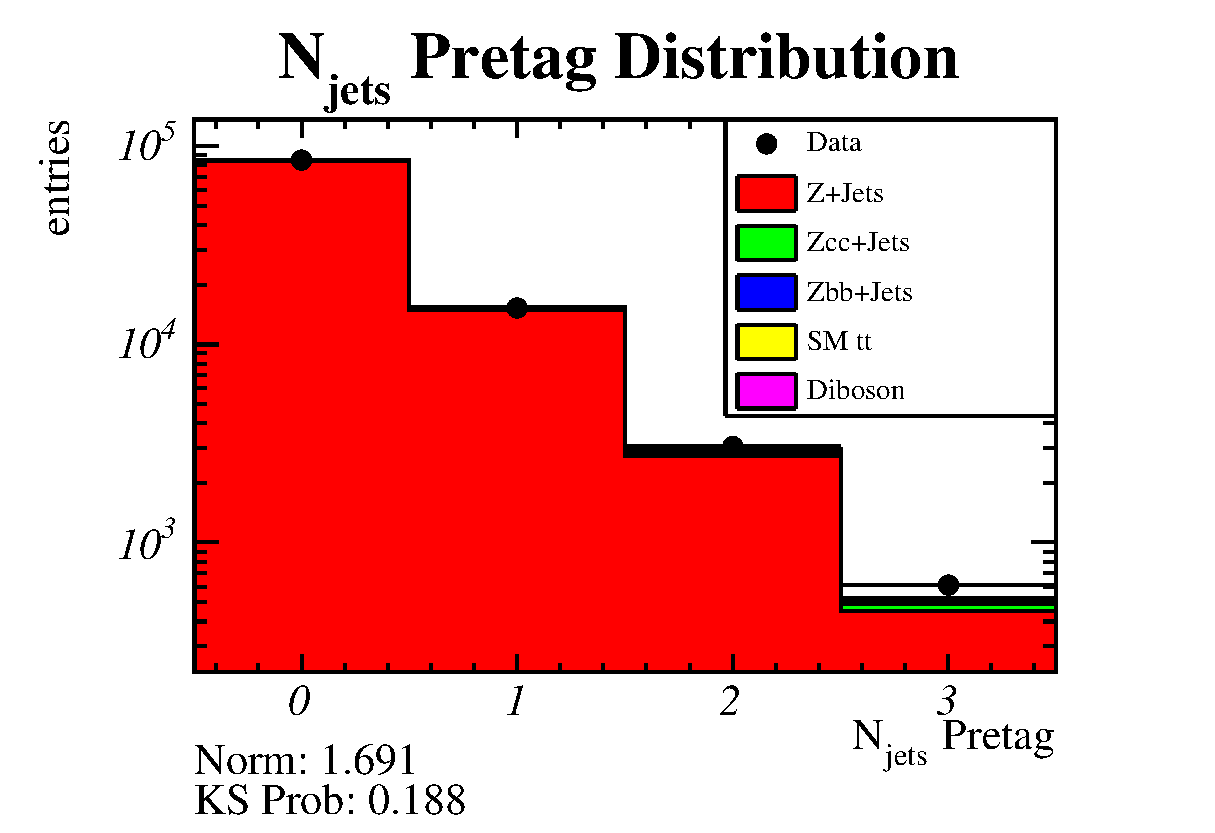
\includegraphics[width=0.48\textwidth]{pics/20070524_njet_nj_pre.eps}}
    \subfigure[]{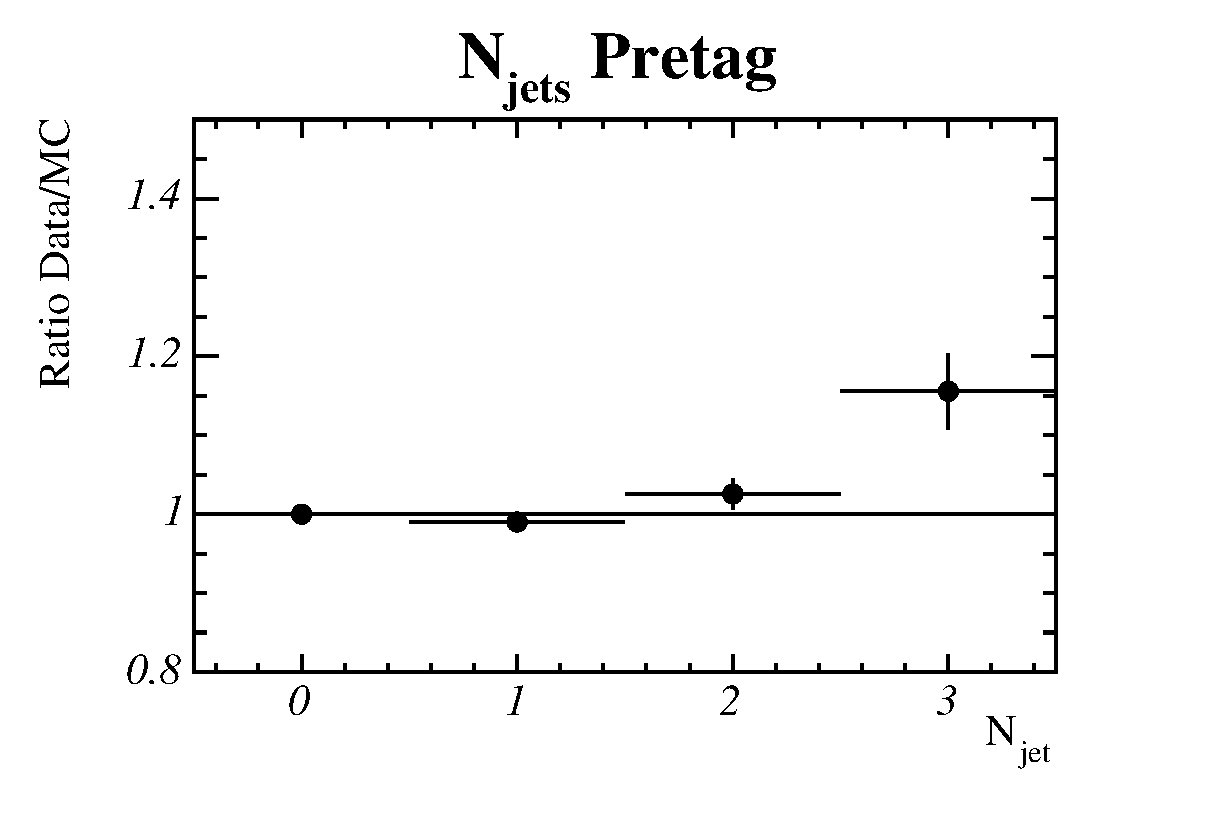
\includegraphics[width=0.48\textwidth]{pics/20070524_njet_ratio_nj_pre.eps}}
  \end{center}
  \caption{Data-MC comparison of the number of jets in events with a
    reconstructed $Z$. (a) Distribution of the number of jets before
    $b$-tagging. (b) ratio of data over MC.}
  \label{fig:alpdata}
\end{figure}

\begin{figure}[t]
  \begin{center}
    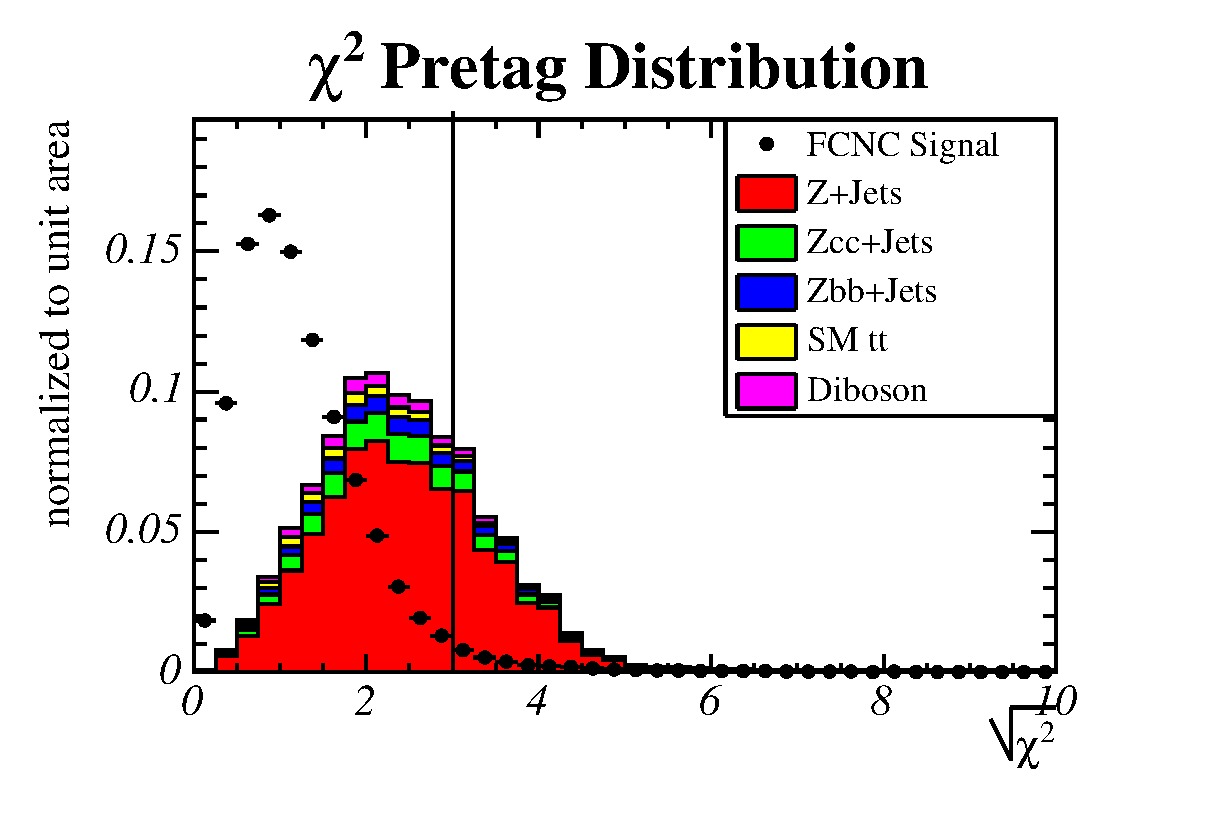
\includegraphics[width=0.6\textwidth]{pics/20070525_chi_pre.eps}
  \end{center}
  \caption{Mass $\chi^2$ distribution of signal and background events. The signal and background samples are normalized to unit area.}
  \label{fig:chi2_separation}
\end{figure}


%In $700\unit{pb^{-1}}$ of
%data, we found 55,775 $Z$ candidates. For $1\unit{fb^{-1}}$, we expect
%80,252 $Z$ candidates. Using the fraction of \Zj in the signal region
%predicted by Monte Carlo, we expect 125 \Zj background events in our
%signal region.


\subsubsection{Heavy Flavor Content and Tagging Rates}
$Z$'s produced in association with heavy flavor ($b$ and $c$) jets
constitute a large portion of the background in the $b$-tagged
sample. We estimate this background by measuring the heavy flavor
fractions, \ie the proportion of \Zj events containing a $b$ or $c$
jet, and the tagging efficiencies for these heavy flavor events. We
measure the contributions to the $b$-tagged background from the MC
samples with $Z+\bbbar+0,1,2$\,partons and $Z+\ccbar+0,1,2$\,partons
and check them in the control region of three or fewer jets in the
data.
%In order to avoid double counting, we discard events
%with heavy flavor in the light flavor samples and events with $b$ jets
%in the $Z$+\ccbar+$n$p samples. The generated \xsects used to weight
%the heavy flavor samples are given in Table~\ref{Znpsigma}. In these
%events, we allow for the possibility of loosing a heavy flavor jet or
%of the two heavy flavor jets merging. 
We divide the sample into events with one heavy flavor jet and events
with two heavy flavor jets. We identify heavy flavor jets by matching
them to $b$ and $c$ hadrons in the OBSP list, as described in
Section~\ref{section:tageff}.  The heavy flavor fractions measured in
the MC simulation are given in Table~\ref{table:Z+HFfrac}.

\begin{table}[t]
\begin{center}
  \caption{\label{table:Z+HFfrac} $Z$ + Heavy Flavor fractions in \alp
    MC. This table gives the fraction of \Zj events (in \%) that
    contain heavy flavor jets, for each physical process, sorted by
    the amount of heavy flavor and number of jets.
    Only statistical errors are given.}
  \vspace{2mm}

  
\small
\begin{tabular}{lD{;}{\pm}{-1}D{;}{\pm}{-1}D{;}{\pm}{-1}D{;}{\pm}{-1}}
\toprule
 {\bf Sample} 
& \multicolumn{1}{c}{\bf 1-jet (\%)}
& \multicolumn{1}{c}{\bf 2-jet (\%)}
& \multicolumn{1}{c}{\bf 3-jet (\%)}
& \multicolumn{1}{c}{\bf 4-jet (\%)} \\
\midrule
$Z\bbbar$, 1 $b$ & 0.8;0.01 & 1.5;0.03 & 2.4;0.05 & 3.3;0.10 \\
$Z\bbbar$, 2 $b$ &  \multicolumn{1}{c}{---} & 1.0;0.02 & 2.1;0.05 & 4.2;0.45 \\
$Z\ccbar$, 1 $c$ & 1.9;0.03 & 3.7;0.07 & 5.5;0.14 & 7.7;0.81 \\
$Z\ccbar$, 2 $c$ &  \multicolumn{1}{c}{---} & 1.4;0.02 & 3.3;0.14 & 5.9;0.17 \\
\bottomrule
\end{tabular}


%   \small\begin{tabular}{lD{;}{\pm}{-1}D{;}{\pm}{-1}D{;}{\pm}{-1}D{;}{\pm}{-1}} \toprule
%     {\bf Sample} & \multicolumn{1}{c}{\bf 1-jet} 
%     & \multicolumn{1}{c}{\bf 2-jet} 
%     & \multicolumn{1}{c}{\bf 3-jet} 
%     & \multicolumn{1}{c}{\bf \boldmath$\geq$\unboldmath 4-jet} \\ 
%     \midrule
%     $Z\bbbar,\, 1\,b$ & 1.5 ; 0.1 & 2.6 ; 0.1 & 3.9 ; 0.2 & 3.8 ; 0.3 \\ 
%     $Z\bbbar,\, 2\,b$ &           & 1.6 ; 0.2 & 3.2 ; 0.3 & 5.6 ; 0.4 \\ 
%     $Z\ccbar,\, 1\,c$ & 0.2 ; 0.0 & 0.5 ; 0.0 & 0.7 ; 0.0 & 1.0 ; 0.1 \\
%     $Z\ccbar,\, 2\,c$ &           & 1.6 ; 0.1 & 3.5 ; 0.1 & 5.7 ; 0.2 \\
%     \bottomrule
%   \end{tabular}
  
\end{center}
\end{table}

We have checked the tagging rates predicted by the \Zj MC simulation
including \Zcc and \Zbb in data.  As the SM \ttbar channels contains
two real $b$ quarks, it contributes significantly to the heavy flavor
content of the background cocktail. To a lesser extend also the
diboson background contributes to the tagging rate. We correct the MC
tagging information by scale factors and mistag probabilities as
described in Section~\ref{section:tageff}. For the comparison we study
the $n$-jet distributions in data and MC simulation.  To keep the
analysis blind, the comparison is restricted to the events with three
or fewer jets.  We keep the contribution from SM \ttbar and diboson
production constant and normalize the \Zj contribution to the pre-tag
data. Fig.~\ref{fig:njet_tag} shows the data-MC comparison. The MC
underestimates the tagging rate in the data by at least 20\%
for all jet bins.

\begin{figure}[t]
  \begin{center}
    \subfigure[]{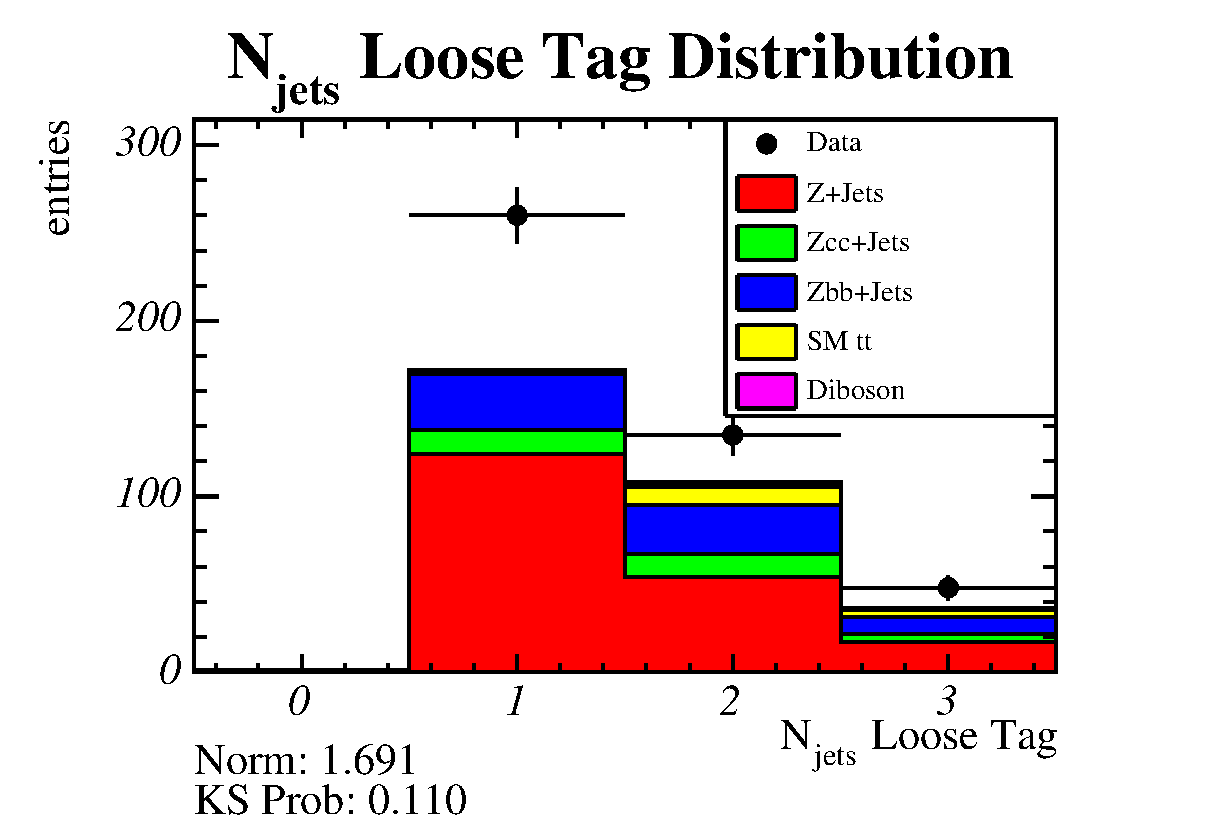
\includegraphics[width=0.48\textwidth]{pics/20070524_njet_nj_loose.eps}}
    \subfigure[]{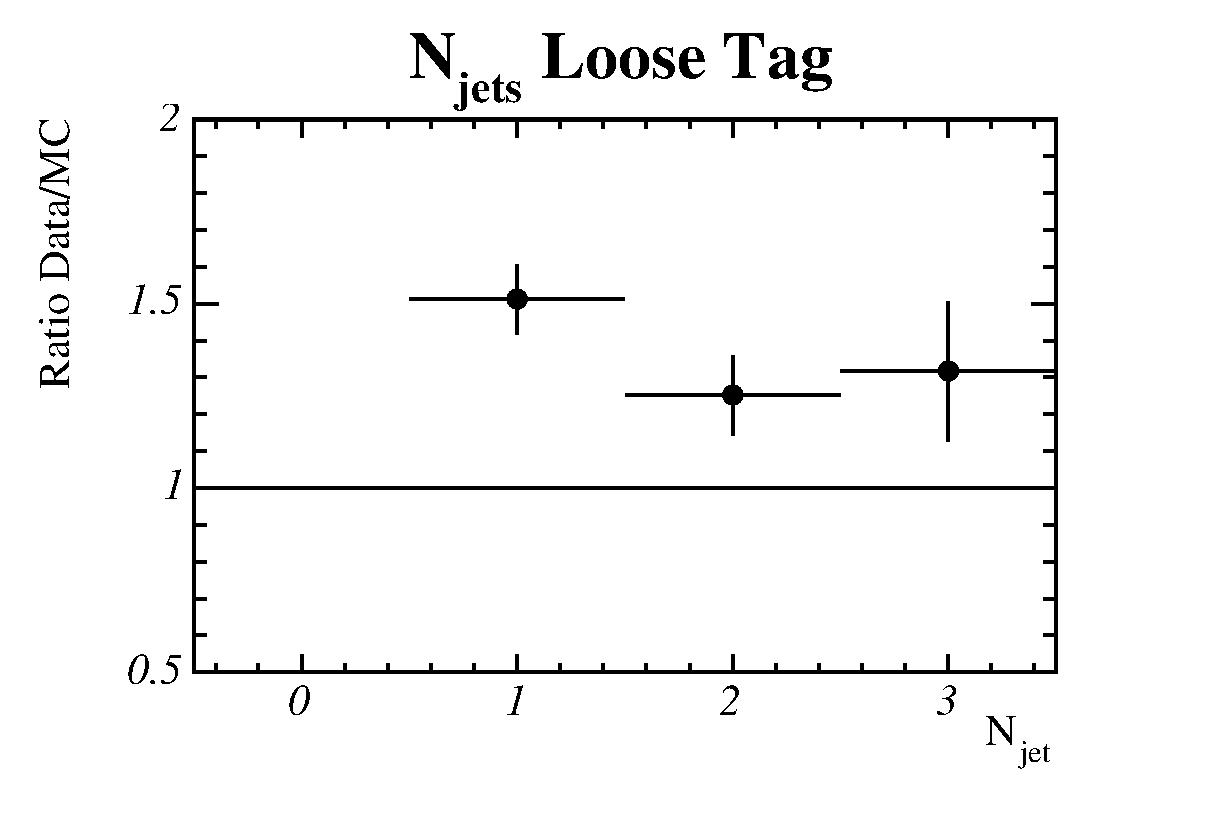
\includegraphics[width=0.48\textwidth]{pics/20070524_njet_ratio_nj_loose.eps}}
  \end{center}
  \caption{Data-MC comparison of the number of tagged events with 1--3
    jets. (a) Distribution of the number of jets for at least one
    loose SECVTX $b$-tag. (b) ratio of data over MC. Note that the MC
    distribution is normalized to the pre-tag data sample.}
  \label{fig:njet_tag}
\end{figure}

The fraction of background events that we expect to be tagged based on
the measurement of heavy flavor fractions in the MC simulation amounts
to 11\%. As we suspect this number to underestimate the real tagging
rate, we double-check it with two different methods. We obtain the
tagging rate from the high-$\chi^2$ sideband by counting the
number of events with a loose SECVTX tag in the region of
$\sqrt{\chi^2}>3$. We count 5 events out of 31, resulting in a tagging
rate of $16\pm7\%$.  As the uncertainty of this data-driven method
is rather large, we check it with a fit to tagging templates.  Tagging
templates are MC templates that contain the MC predictions of the
tagging probabilities separately for the number of jets in the event
and the number of $b$-tags for all background samples and both the
loose and the tight tagger.  Fits to the templates allow subsets of
these degrees of freedom to float. Knowing that the MC does not
predict the jet multiplicities well, we let every jet bin float. The
contribution of SM \ttbar is fixed, the light flavor \Zj sample and
the combination of the \Zcc and the \Zbb samples are allowed to float.
The data together with the fitted template are shown in
Fig.~\ref{fig:tagtemp}. We extract a tagging rate of 14\% from 
this method. We use the average of the results from the $\chi^2$ method
and the template fitting method as our prediction for the 
tagging rate and conservatively estimate the uncertainty such that the
11\% result from the MC heavy flavor fractions is covered:
$15 \pm 4\%$.


\begin{figure}[t]
  \begin{center}
    \subfigure[]{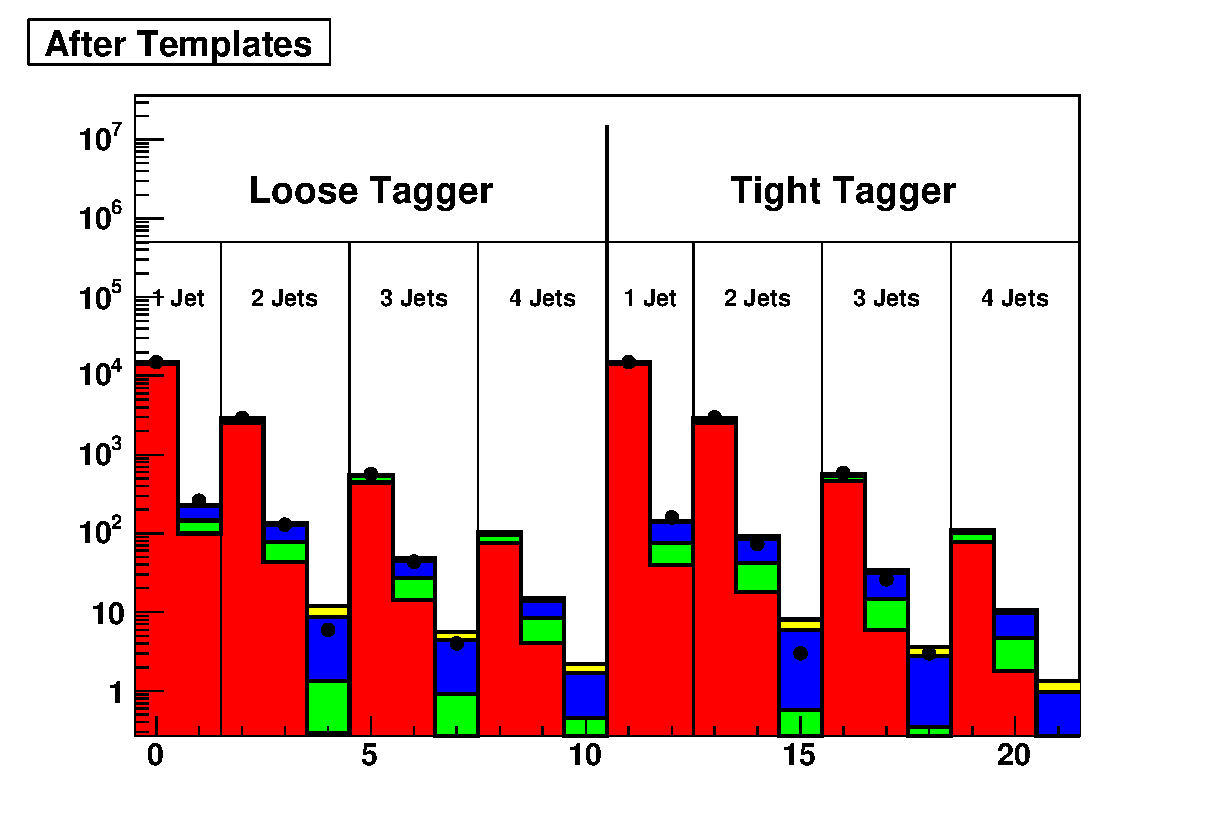
\includegraphics[width=0.48\textwidth]{pics/jettag_Ulrich_hf_after.eps}}
    \subfigure[]{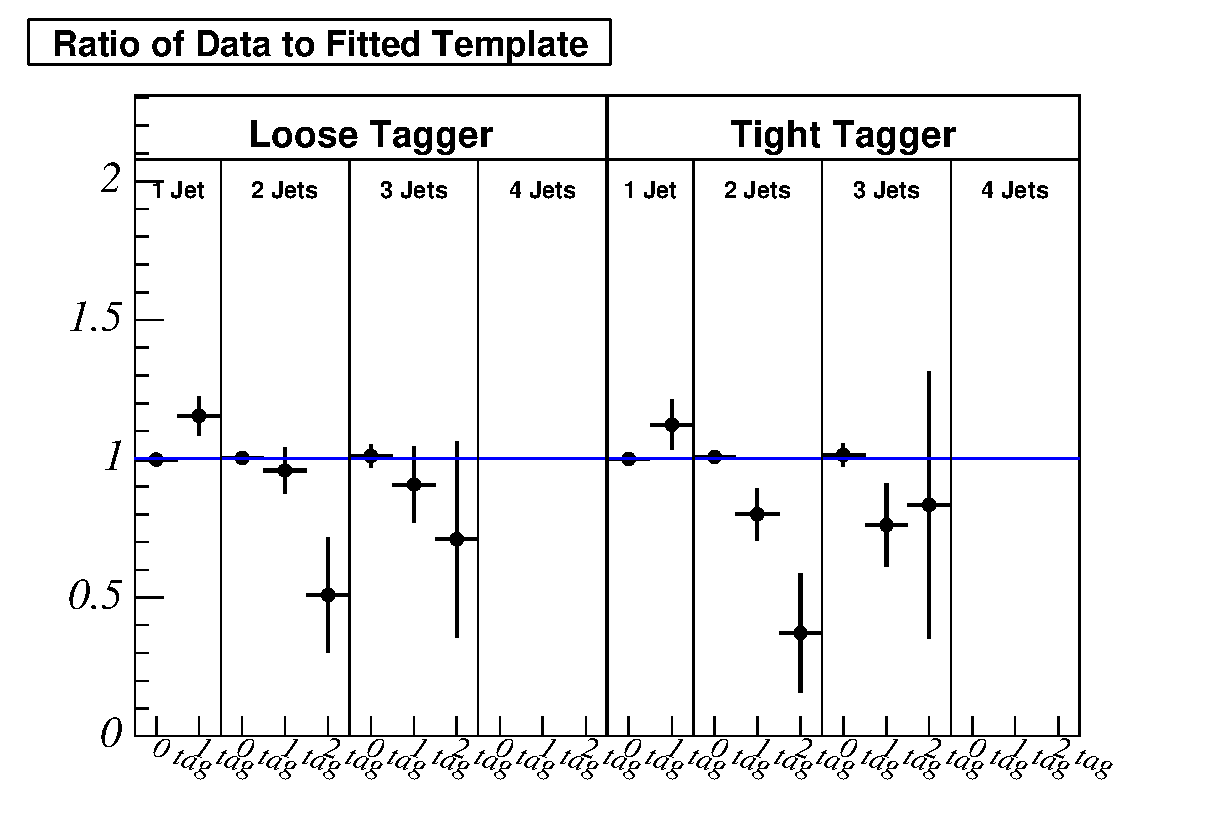
\includegraphics[width=0.48\textwidth]{pics/jettag_Ulrich_hf_ratio.eps}}
  \end{center}
  \caption{Extraction of tagging fractions from a fit to tagging templates. (a) tagging templates fitted to data. (b) Ratio }
  \label{fig:tagtemp}
\end{figure}



%NEEDS UPDATE!!!
%We measure the raw tagging efficiencies for the heavy flavor events in
%the MC simulation for $Z\bbbar$ and $Z\ccbar$ events with one or two
%heavy flavor jets as a function of the jet multiplicity.  The tagging
%efficiencies are then corrected in the same manner as for the signal
%MC, as described in Section~\ref{section:tageff}, \ie taking into
%account $b$-tagging scale factors for identified heavy flavor jets and
%the mistag matrix including $\alpha\beta$ corrections for light flavor
%jets.  The resulting expected tagging efficiencies for heavy flavor
%events in the data are given in Table~\ref{table:HFtagrate}.

%The tagging efficiencies for the heavy flavor events are measured in
%in the MC for each class of events then scaled in a similar manner
%to the tagging efficiency in signal Monte Carlo. The tags in $b$ and
%$c$ jets are scaled down by the loose SECVTX scale factor. In
%addition, light flavor tags are also allowed by adding tags in the
%light flavor jets based on the mistag matrix prediction. This prevents
%the double counting of heavy flavor events with mistags as both heavy
%flavor events and mistag events. 


% \begin{table}[t]
% \begin{center}
%   \caption{\label{table:HFtagrate} Expected $b$-tagging efficiencies
%     in the data (in \%) for $Z$ + Heavy Flavor events, corrected for
%     tagging scale factors and including light flavor tags. Only
%     statistical errors are given.}
%   \vspace{2mm}
  
%   \small\begin{tabular}{lD{;}{\pm}{-1}D{;}{\pm}{-1}D{;}{\pm}{-1}D{;}{\pm}{-1}} \toprule
%     {\bf Sample} & \multicolumn{1}{c}{\bf 1-jet} 
%     & \multicolumn{1}{c}{\bf 2-jet} 
%     & \multicolumn{1}{c}{\bf 3-jet} 
%     & \multicolumn{1}{c}{\bf \boldmath$\geq$\unboldmath 4-jet} \\ 
%     \midrule
%     $Z\bbbar,\, 1\,b$ & 31 ; 2 & 36 ; 3 & 38 ; 4 & 44 ; 6 \\
%     $Z\bbbar,\, 2\,b$ &        & 55 ; 7 & 60 ; 8 & 60 ; 7 \\ 
%     $Z\ccbar,\, 1\,c$ &  9 ; 1 & 11 ; 1 & 14 ; 2 & 15 ; 5 \\
%     $Z\ccbar,\, 2\,c$ &        & 16 ; 1 & 18 ; 1 & 22 ; 1 \\
%     \bottomrule
%   \end{tabular}
% \end{center}
% \end{table}

% In order to obtain the total expected tag rates for \Zj events in the
% data, we multiply the $Z$ + Heavy Flavor fractions and the expected
% tagging efficiencies.  The resulting expected tag rates for \Zj events
% are summarized in Table~\ref{table:Z+Jets_tagrates}.

% \begin{table}
%   \begin{center}
%     \caption{\label{table:Z+Jets_tagrates} The expected tag rates for
%       \Zj events in each $n$-jet bin based on measurements in the MC
%       simulation.}
%     \vspace{2mm}
    
%     \small\begin{tabular}{lD{;}{\pm}{-1}} 
%       \toprule
%       {\bf Sample} & \multicolumn{1}{c}{\bf Expected Tag Rate (\%)} \\ 
%       \midrule
%       $Z+1$\,jet       & 0.5 ; 0.1 \\ 
%       $Z+2$\,jets      & 2.1 ; 0.2 \\
%       $Z+3$\,jets      & 3.9 ; 0.4 \\
%       $Z+\geq 4$\,jets & 6.7 ; 0.5 \\ 
%       \bottomrule
%     \end{tabular}
%   \end{center}
% \end{table}

% In order to verify that the expected tag rate for our signal region
% ($Z+\geq4$\,jet events) is correct, we check the expected tag rates
% for the control region ($Z+1,2,3$\,jet events) against tag rates in
% data. We used the full dataset up to the September 2005 shutdown,
% which is about $695\invpb$ of data. We directly measured the tag rates
% and mistag rates in data. 
% % The measurement of mistag rates in data is described in detail in
% % the next section.
% We also double-check the tag rates and mistag rates for the tight
% tagger against the loose tagger to give us an additional constraint on
% checking the heavy flavor content of the data versus the MC
% simulation. The difference between the tag rate and mistag rate gives
% the rate of tagged heavy flavor events in data. The tag rates, mistag
% rates, and the differences between the two for the loose SECVTX tagger
% are given in Table~\ref{table:loose_datatag} and the tag rates, mistag
% rates and the differences between the two for the tight tagger are
% given in Table~\ref{table:tight_datatag}.  We compared the differences
% in tag rates and mistag rates to the expected tag rate due to heavy
% flavor predicted by Monte Carlo, given in
% Table~\ref{table:Z+Jets_tagrates}. The ratios between data tag rates
% and Monte Carlo predictions are given in
% Table~\ref{table:data_MC_ratios}.

% THE FOLLOWING NEEDS TO BE REVISITED:
% The ratios for the loose and tight
% taggers in events with different number of jets are consistent with
% each other within one sigma and consistently higher than 1.0. The
% average ratio is $1.51 \pm 0.17$. Scaling the predicted tag rate in
% the signal region ($Z\geq 4$\,jet events) by a factor of 1.51 gives a
% rate of $10.12 \pm 1.37\%$. We expect $8.6 \pm 1.12$ tagged events in
% our signal region resulting from $Z$'s produced in association with
% $b$ and $c$ jets.

% \begin{table}[h]
%   \begin{center}
%     \caption{\label{table:loose_datatag} The tag rates, mistag rates, and the differences between the two for the loose SECVTX tagger in \Zj data.}
%     \vspace{2mm}
    
%     \small\begin{tabular}{lD{;}{\pm}{-1}D{;}{\pm}{-1}D{;}{\pm}{-1}} 
%       \toprule
%       {\bf Sample} 
%       & \multicolumn{1}{c}{\bf Tag Rate (\%)}
%       & \multicolumn{1}{c}{\bf Mistag Rate (\%)} 
%       & \multicolumn{1}{c}{\bf Difference (\%)}\\
%       \midrule
%       $Z+1$\,jet & 1.57 ; 0.13 & 0.70 ; 0.11 & 0.87 ; 0.17 \\
%       $Z+2$\,jets & 4.84 ; 0.52 & 1.74 ; 0.26 & 3.10 ; 0.58 \\
%       $Z+3$\,jets & 8.01 ; 1.43 & 3.12 ; 0.47 & 4.89 ; 1.51 \\
%       \bottomrule
%     \end{tabular}
    
%   \end{center}
% \end{table}

% \begin{table}[h]
%   \begin{center}
%     \caption{\label{table:tight_datatag} The tag rates, mistag rates, and the differences between the two for the tight SECVTX tagger in \Zj data.}
%     \vspace{2mm}
    
%     \small\begin{tabular}{lD{;}{\pm}{-1}D{;}{\pm}{-1}D{;}{\pm}{-1}}
%       \toprule
%       {\bf Sample} 
%       & \multicolumn{1}{c}{\bf Tag Rate (\%)}
%       & \multicolumn{1}{c}{\bf Mistag Rate (\%)} 
%       & \multicolumn{1}{c}{\bf Difference (\%)}\\
%       \midrule
%       $Z+1$\,jet & 1.07 ; 0.11 & 0.26 ; 0.04 & 0.81 ; 0.12 \\ 
%       $Z+2$\,jets & 2.76 ; 0.39 & 0.68 ; 0.10 & 2.08 ; 0.40 \\
%       $Z+3$\,jets & 6.35 ; 1.28 & 1.43 ; 0.21 & 4.92 ; 1.30 \\
%       \bottomrule
%     \end{tabular}
%   \end{center}
% \end{table}

% \begin{table}[h]
%   \begin{center}
%     \caption{\label{table:data_MC_ratios} The ratios between tag rates from heavy flavor in data and Monte Carlo for loose and tight SECVTX taggers.}
%     \vspace{2mm}
    
%     \small\begin{tabular}{lD{;}{\pm}{-1}D{;}{\pm}{-1}}
%       \toprule
%       {\bf Sample}
%       & \multicolumn{1}{c}{\bf Ratio (Loose Tagger)}
%       & \multicolumn{1}{c}{\bf Ratio (Tight Tagger)} \\ 
%       \midrule
%       $Z+1$\,jet & 1.67 ; 0.45 & 1.88 ; 0.52 \\ 
%       $Z+2$\,jets & 1.48 ; 0.31 & 1.20 ; 0.27 \\
%       $Z+3$\,jets & 1.27 ; 0.41 & 1.57 ; 0.46 \\
%       \bottomrule
%     \end{tabular}
%   \end{center}
% \end{table}

% \subsubsection[$Z$ + Light Flavor]{\boldmath $Z$\unboldmath{} + Light Flavor}
% Contributions to the tagged background can also result from $Z$'s
% produced in association with light flavor jets, where these jets have
% been mistagged. Although the rate for mistagging light flavor jets is
% small, there are many more events in \Zj events with only light flavor
% jets than events with heavy flavor jets, so a significant portion of
% the tagged background is from $Z$ + Light Flavor events. We estimate
% the mistag probability per event using the mistag matrix and the
% $\alpha\beta$ correction as described in Section~\ref{section:tageff}.
% The average event mistag probabilities for $Z+1,2,3$\,jet events are
% given in Table~\ref{table:loose_datatag} for the loose SECVTX tagger
% and in Table~\ref{table:tight_datatag} for the tight SECVTX tagger.

% THE FOLLOWING NEEDS TO BE REVISITED:
% We extrapolate these mistag rates into our signal region of four or
% more jets (HOW???) and estimate that 6\% of the $Z+\geq 4$\,jet events
% which have only light flavor jets will be tagged (TIGHT TAGGER???). We
% expect 24.3\% of the $Z+\geq 4$\,jet events to contain heavy flavor
% jets (MC estimate + 50\% scaling based on data), i.e. we expect 64 $Z$
% + Light flavor background events in our signal region. Of these, we
% expect 3.9 events to be tagged.
	
%In order to get an estimate for the background from mistagged light
%flavor jets, we ran the {\it negative mistag matrix} on the \Zj sample
%and then apply the rates to the portion of \Zj events which have only
%light flavor jets. The mistag matrix determines the probability for a
%light jet to be tagged by applying the generic jet tag rate to jets in
%the \Zj sample. Details on the mistag matrix are given in CDF Note
%7326~\cite{CDF7326}. This estimate is further corrected by the $\Sigma
%E_{T}$-dependent {\it mistag asymmetry}($\alpha \beta$). These
%corrections account for the imbalance in positive and negative tags
%for light jets and the effect of heavy flavor tags in the generic jet
%samples from which the mistag matrix was derived. More information on
%these corrections can be found in~CDF Note 7585~\cite{CDF7585}.

%Once a mistag probability has been assigned to each jet, we can
%calculate the probability for getting $\geq$1 mistagged jet in each
%event. We do this by subtracting the product of probabilities that
%each jet in the event will not be mistagged from one, i.e.  $1 - \Pi
%(1 - P_{i})$ where $P_i$ is the mistag probability for the
%$i^\mathrm{th}$ jet. 

\subsection[Standard Model \ttbar]{Standard Model \boldmath\ttbar\unboldmath}
Another background contribution to our FCNC search
originates from standard model decays of \ttbar pairs ($\ttbar
\to \Wp b\, \Wm \bbar$). Although there are no real $Z$'s in these
events, the two leptons in dilepton decays can have an invariant mass
reconstructed within our $Z$ mass window. In addition, in lepton+jets
events, a jet can be misidentified as a lepton. These events
contribute if the dilepton mass falls within our $Z$ mass window.

For our studies of the SM \ttbar background, we used 4.7 million
MC-simulated $t\bar{t}$ events generated with the \pyth event
generator at a top quark mass of 175\gevcsq (MC sample:
\texttt{ttop75}). We use the measured \ttbar production \xsect in the
lepton+jets channel using SECVTX $b$-tagged events of $8.8 \pm
1.1\unit{pb}$~\cite{CDF8767} to normalize the MC predictions to
1.12\invfb. The normalized dilepton mass spectrum obtained from the SM
\ttbar MC sample is shown in Fig.~\ref{fig:dilepmass_SMtop}a.  Although
there is no $Z$ mass peak, there are events with a reconstructed
dilepton mass that falls within the $Z$ mass window. The solid line in
Fig.~\ref{fig:dilepmass_SMtop}b shows the distribution of the number of
jets for events inside the $Z$ mass window.  Most of these events have
fewer than four jets. This is because in dilepton events, there are
only two extra hard jets from the decay of the \ttbar pair and in
lepton+jets events, one jet is misidentified as a lepton so there are
only three jets left over. To pass the requirements of four or more
jets, the events need to have extra jets from initial state and final
state radiation. Therefore, the $\geq 4$ jet requirement rejects
91.7\% of this background. Fig.~\ref{fig:dilepmass_SMtop}a shows the 
reconstructed dilepton mass also after requiring $\geq$4 jets. This leaves 
us with $2.4\pm 0.3$ expected events in the signal region in 1.12\invfb, 
rendering SM \ttbar a much smaller background than \Zj ($135\pm 28$ events).


\begin{figure}[t]
  \begin{center}
    \subfigure[]{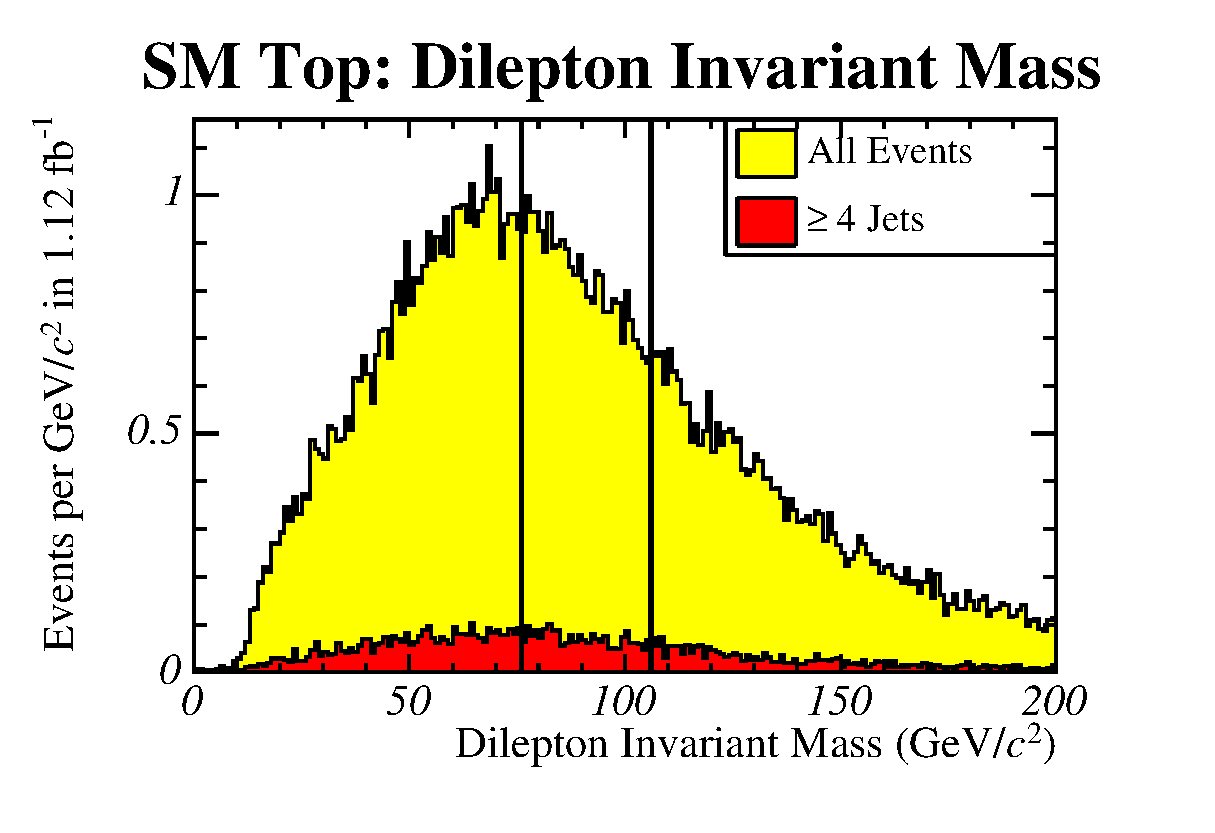
\includegraphics[width=0.48\textwidth]{pics/20070413_smtt_dilepton_mass.eps}}
    \subfigure[]{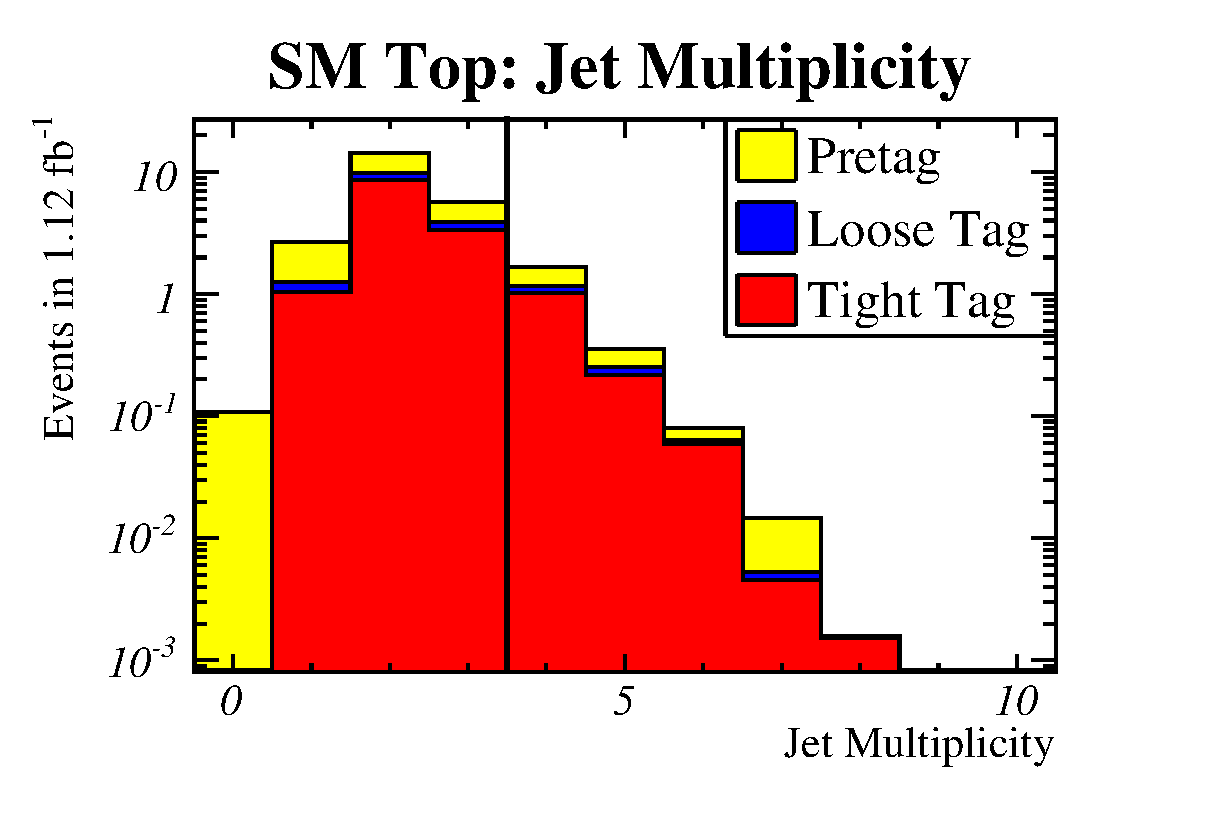
\includegraphics[width=0.48\textwidth]{pics/20070413_smtt_jetmult_tagger.eps}}
  \end{center}
  
  \caption{(a) Reconstructed dilepton mass for all standard model
    \ttbar MC events and events with $\geq 4$~jets. The vertical lines
    show our $Z$ mass selection window. (b) Jet multiplicity for
    standard model \ttbar MC events before $b$-tagging and using the
    loose and tight SECVTX tagger.}
  \label{fig:dilepmass_SMtop}
\end{figure}


Although the contribution of SM \ttbar events to the untagged
background is small, we have to take into account the fact that 
that these events have two $b$-jets in the final state. The efficiency for
finding a $b$-tag is therefore much higher compared to \Zj. As described for the
FCNC signal MC in Section~\ref{section:tageff}, the $b$- and $c$-jet
tags are scaled down by the scale factor, and light flavor tags are
added according to mistag matrix predictions to produce an expected
tagging efficiency in data. In 1.12\invfb of data, we expect $1.6\pm
0.2$ SM \ttbar background events with a loose SECVTX $b$-tag
(compared to an expected number of $20 \pm 6$ tagged \Zj events 
for the loose SECVTX tagger). These results and the MC sample used are
summarized in Table~\ref{table:small_backgrounds}.

\subsection{Dibosons}
We expect background contributions similar to SM \ttbar production
from the production of pairs of gauge bosons (``diboson''), 
$WZ$ and $ZZ$, where events contain real $Z$'s that can
decay into leptons while the other boson is allowed to decay to a pair
of jets, including heavy flavor jets.  Within the detector resolution,
the dijet invariant mass is indistinguishable from the $W$ mass in the
signal MC. There can also be additional jets from initial and final
state radiation which will make these events fall in our signal region
of $Z+4$\,jets.  

We used MC events simulated with \pyth and normalized to the
theoretical \xsects for diboson production to estimate this
background. The theoretical \xsects and their uncertainties are
obtained from the MCFM event generator using MRS98 parton distribution
functions~\cite{Campbell:1999ah}. The samples and \xsects for these
backgrounds are given in Table~\ref{table:small_backgrounds}, along with 
the number of events in 1.12\invfb, before and after tagging. The total
background from both $WZ$ and $ZZ$ diboson production before $b$-tagging 
amounts to $2.9\pm 0.1$ events, larger than the background from SM \ttbar
production. Due to the small fraction of heavy flavor jets, the
diboson background is suppressed in the tagged analysis compared to SM
\ttbar production, with an expected $0.4 \pm 0.0$ events using the
loose SECVTX tagger.

\begin{table}
\small
\begin{center}
\caption{\label{table:small_backgrounds} The dataset names, \xsects, number of events 
  in the MC sample, and expected number of events in 1.12\invfb for both the SM
  \ttbar and the $WZ$ and $ZZ$ diboson samples. Also included in the uncertainty
  calculation is the 6\% luminosity uncertainty.}
\vspace{2mm}

\begin{tabular}{c c D{;}{\pm}{-1} D{;}{,}{-1} D{;}{\pm}{-1} D{;}{\pm}{-1} } 
\toprule
\multicolumn{1}{c}{\bf Sample} & 
\multicolumn{1}{c}{\bf Dataset} & 
\multicolumn{1}{c}{\bf Cross Section} & 
\multicolumn{1}{c}{\bf Generated} &
\multicolumn{1}{c}{\bf Events} &
\multicolumn{1}{c}{\bf Events w/ Loose} \\ 
 & 
\multicolumn{1}{c}{\bf Name} & 
\multicolumn{1}{c}{\bf (pb)} &
\multicolumn{1}{c}{\bf Events} & 
\multicolumn{1}{c}{\bf Pre-Tagged} & 
\multicolumn{1}{c}{\bf SECVTX $b$-Tag} \\

\midrule
SM \ttbar & ttop75 & 8.5;1.1   & 4,719;385 & 2.4;0.3 & 1.6;0.2 \\
$WZ$      & itopwz & 3.96;0.06 & 2,340;145 & 2.0;0.1 & 0.2;<0.1 \\
$ZZ$      & itopzz & 1.58;0.02 & 2,323;812 & 0.8;0.1 & 0.2;<0.1 \\
\bottomrule
\end{tabular}    

  \end{center}
\end{table}

%\begin{table}
%  \begin{center}
%    \caption{\label{table:diboson_bkg} Expected number of background events from %diboson production in 1.12\invfb, before and after $b$-tagging.}
%    \vspace{2mm}%%

%    \small
%    \begin{tabular}{lD{;}{\pm}{-1}D{;}{\pm}{-1}D{;}{\pm}{-1}} \toprule
%      \multicolumn{1}{l}{\bf Sample} & 
%      \multicolumn{1}{c}{\bf Without \boldmath\btag\unboldmath} &
%      \multicolumn{1}{c}{\bf Loose SECVTX \boldmath\btag\unboldmath} &
%      \multicolumn{1}{c}{\bf Tight SECVTX \boldmath\btag\unboldmath} \\
%      \midrule
%      $WW$  & 0.08 ; 0.02 & 0.03 ; 0.01 & 0.03 ; 0.01 \\
%      $WZ$  & 2.15 ; 0.07 & 0.25 ; 0.02 & 0.14 ; 0.02 \\
%      $ZZ$  & 0.89 ; 0.03 & 0.18 ; 0.01 & 0.14 ; 0.01 \\
%      \midrule
%      Total & 3.12 ; 0.08 & 0.45 ; 0.03 & 0.30 ; 0.02\\
%      \bottomrule
%    \end{tabular}
%  \end{center}
%\end{table}

\subsection[$W$ + Jets]{\boldmath $W$\unboldmath{} + Jets}
Another source of background to the FCNC signal comes from the
production of $W$'s in association with jets, \Wj. \Wj events are 
abundant at CDF; the ratio of the \xsects of $W+(n+1)$ jets to 
$Z+n$ jets is approximately 60\%~\cite{TopXSec}. Unlike
the \Zj background, \Wj events require the charged lepton from 
the decay $W\to\ell\nu$ and a jet misidentified as a lepton to 
reconstruct with an invariant mass within the $Z$ mass window. 
Factoring in the probability that this jet becomes
misidentified as lepton decreases this background with respect to
\Zj even further.

We employ different methods to estimate the background from \Wj events
in \ee and \mm final states.  For dimuon events, it is sufficient to
estimate the number of background events from the number of same-sign
muon pairs (or muon-track pairs) that fall into the $Z$ mass window.
We found only 15 same-sign $Z$ candidates in a sample corresponding to
$700\invpb$ of integrated luminosity. None of the events contained
four or more jets; therefore, we conclude that the background from
$W\rightarrow \mu\nu$ + jets events is negligible for our analysis.  
For the electron sample, using same-sign $Z$ candidates is not sufficient 
to estimate the \Wj background. There is a significant contributions to 
the same-sign $Z$ candidates from phoenix electrons whose charge sign was
misidentified. In addition, bremsstrahlung photons radiated from one
or both electrons from the $Z$ decay can be converted into \ee pairs
in the detector material (``trident electrons''), such that three electron 
tracks can be reconstructed per $Z$ leg. One of the electrons has
opposite charge to the original electrons.  We use both the data and
the MC simulation to predict the number of same sign \Zee events we
expect.

The main technique to estimate the \Wj background in \Zee is to study
same-sign electron-muon pairs with an invariant mass falling into the
our $Z$ mass window.  The dominant source of same-sign $e\mu$ pairs is
\Wj decays in which the $W$ decays into $\mu\nu$ and one of the jets
is misidentified as an electron. The charge sign of the muon can be
trusted because the background in \Zmm is negligible. We expect the
same number of same-sign and opposite-sign $e\mu$ pairs from these
decays. To infer the number of same sign \ee pairs from the number of
same-sign $e\mu$ pairs, we have to take into account that the
acceptances for muon identification are different than those for
electron identification. We scale the number of events we find in the
full 1.12\invfb dataset by the ratio $\mathcal{R}$ of the acceptances
$\mathcal{A}$ for $W$ decays into $e\nu$ and $\mu\nu$ final
states~\cite{Acosta:2004uq}:

\begin{equation}
{\mathcal R} = 
\frac{ {\mathcal A}( W \rightarrow e \nu ) }
{{\mathcal A} ( W \rightarrow \mu \nu ) } = 1.217 \pm 0.026.
\end{equation}

The expected number of background events are compared to the number of
opposite-sign \Zee for three and fewer jets in
Table~\ref{table:wjets_bkg}. The fraction of such events is $6\times
10^{-4}$ such that they can be safely neglected.  Note that our method
to estimate the \Wj background does not include track leptons. We
believe that our conclusion that the \Wj background is negligible is
not changed if track leptons are included.

\begin{table}
  \begin{center}
    \caption{\label{table:wjets_bkg} Expected number of events from
      \Wj production in 1.12\invfb in events with three or fewer jets,
      before and after $b$-tagging. The number is estimated from the
      number of same-sign $e\mu$ pairs in the data and compared to the
      number of opposite-sign (OS) \Zee candidates.}
    \vspace{2mm}

    \small
    \begin{tabular}{lD{;}{\pm}{-1}D{;}{\pm}{-1}D{;}{\pm}{-1}D{,}{,}{-1}} \toprule
      \multicolumn{1}{l}{\bf Sample} & 
      \multicolumn{1}{c}{\bf Without \boldmath\btag\unboldmath} &
      \multicolumn{1}{c}{\bf Loose \boldmath\btag\unboldmath} &
      \multicolumn{1}{c}{\bf Tight \boldmath\btag\unboldmath} &
      \multicolumn{1}{c}{\bf OS \boldmath\Zee\unboldmath} \\
      \midrule
      CEM   &  2.4 ; 1.7 & 0.02 ; 0.16 & \multicolumn{1}{c}{not detectable} & 19,325 \\
      PHX   & 21.9 ; 5.2 & 0.04 ; 0.19 & \multicolumn{1}{c}{not detectable} & 22,107 \\
      \midrule
      Total & 24.3 ; 5.5 & 0.06 ; 0.25 & \multicolumn{1}{c}{not detectable} & 41,432 \\
      \bottomrule
    \end{tabular}
  \end{center}
\end{table}

We have double-checked the results of our \Wj background estimate by
two alternative methods that rely more on MC simulations. For both
methods we use an inclusive \Zee MC sample generated with \pyth
(\texttt{zewk6d}) to subtract the number of same-sign $Z$ candidates
expected from charge misidentification and tridents in real \Zee events
from the number of same-sign $Z$ candidates in the data.  In the first
method we obtain the ratio of same-sign to opposite-sign $Z$
candidates from the MC simulation,

\begin{equation}
N_{\mathrm{bkg}}^\mathrm{data} = N_{Z,\mathrm{SS}}^\mathrm{data} - \frac{N_{Z,\mathrm{SS}}^\mathrm{MC}}{N_{Z,\mathrm{OS}}^\mathrm{MC}} \cdot N_{Z,\mathrm{OS}}^\mathrm{data}.
\end{equation}

For the second method we assume that the fraction of tridents in the same-sign $Z$ candidates is correctly modeled in the MC simulation:

\begin{equation}
N_{\mathrm{bkg}}^\mathrm{data} = N_{Z,\mathrm{SS}}^\mathrm{data} - \frac{N_{Z,\mathrm{SS}}^\mathrm{MC}}{N_{\mathrm{trident,OS}}^\mathrm{MC}} \cdot N_{\mathrm{trident,OS}}^\mathrm{data}.
\end{equation}

We find expected background rates of 0.01--0.04 with these methods,
more than an order of magnitude larger than the result obtained with
our main technique. Note however that these methods are conservative
because both the effects of charge misidentification and the amount of
material in the detector giving rise to tridents tend to be
underestimated in the MC. The conclusion that the \Wj background is
negligible remains valid.

\subsection{Background Summary}
In summary, the main background for the search for the FCNC decay \tZq
comes from $Z$ boson production in association with jets. We found
that the background coming from SM \ttbar production and diboson
production is small, and contributions from \Wj events are
negligible. The expected number of background events in our 1.12\invfb
dataset is summarized in Table~\ref{table:bkg_summary}.


\begin{table}
  \begin{center}
    \caption{\label{table:bkg_summary} Summary of all background
      contributions to the search for the FCNC decay \tZq. Given are
      the expected numbers of background events in 1.12\invfb.}
    \vspace{2mm}

    \small
    \begin{tabular}{lD{;}{\pm}{-1}D{;}{\pm}{-1}D{;}{\pm}{-1}} \toprule
      \multicolumn{1}{l}{\bf Source} & 
      \multicolumn{1}{c}{\bf Without \boldmath\btag\unboldmath} &
      \multicolumn{1}{c}{\bf Loose SECVTX\boldmath\btag\unboldmath} \\
      \midrule
      \Zj                   & 135;28      & 20 ; 6  \\ 
      Standard Model \ttbar & 2.4 ; 0.3 & 1.6  ; 0.2 \\
      Diboson               & 2.8 ; 0.1 & 0.4  ; <0.1 \\
      \Wj                   & \multicolumn{1}{c}{$<0.1$} 
      & \multicolumn{1}{c}{negligible}\\
      \bottomrule
    \end{tabular}
  \end{center}
\end{table}
